\section{Introduction}

For over two years, the COVID-19 pandemic has been a headline research topic as it inescapably invades our world and affects our lives in unparalleled ways. COVID-19 is a disease caused by severe acute respiratory
syndrome coronavirus 2 (SARS-CoV-2), a virus believed have
zoonotic origins \cite{Andersen2020}.

Since its discovery, SARS-CoV-2 studies have identified a range of animal hosts --- including some nonhuman primates,  mustelids, bats, and felines --- that can be infected by and can transmit the virus \cite{Luan2020,Woolsey2020,OIE2022,OudeMunnink2021,Schlottau2020,Sreenivasan2020,Leroy2020}. Conversely, certain research has supported the conclusion that other species (e.g. the domestic pig) are explicitly immune to the virus \cite{Luan2020,Sreenivasan2020,Zhao2020,Shi2020}. This disjunction promotes the question: \emph{what makes some species susceptible to the virus and others immune?} Investigating this question has been an ongoing focus in bioinformatics to mitigate interspecies transmission.

The answer might correspond to how the the virus interacts with its target protein in different hosts. The SARS-COV-2 spike protein’s target is the angiotensin-converting enzyme 2 (ACE2). Differences in the ACE2 sequence can affect the spike protein’s binding affinity, thus affecting the host’s susceptibility to the virus.

\begin{figure}[h]
    \centering
    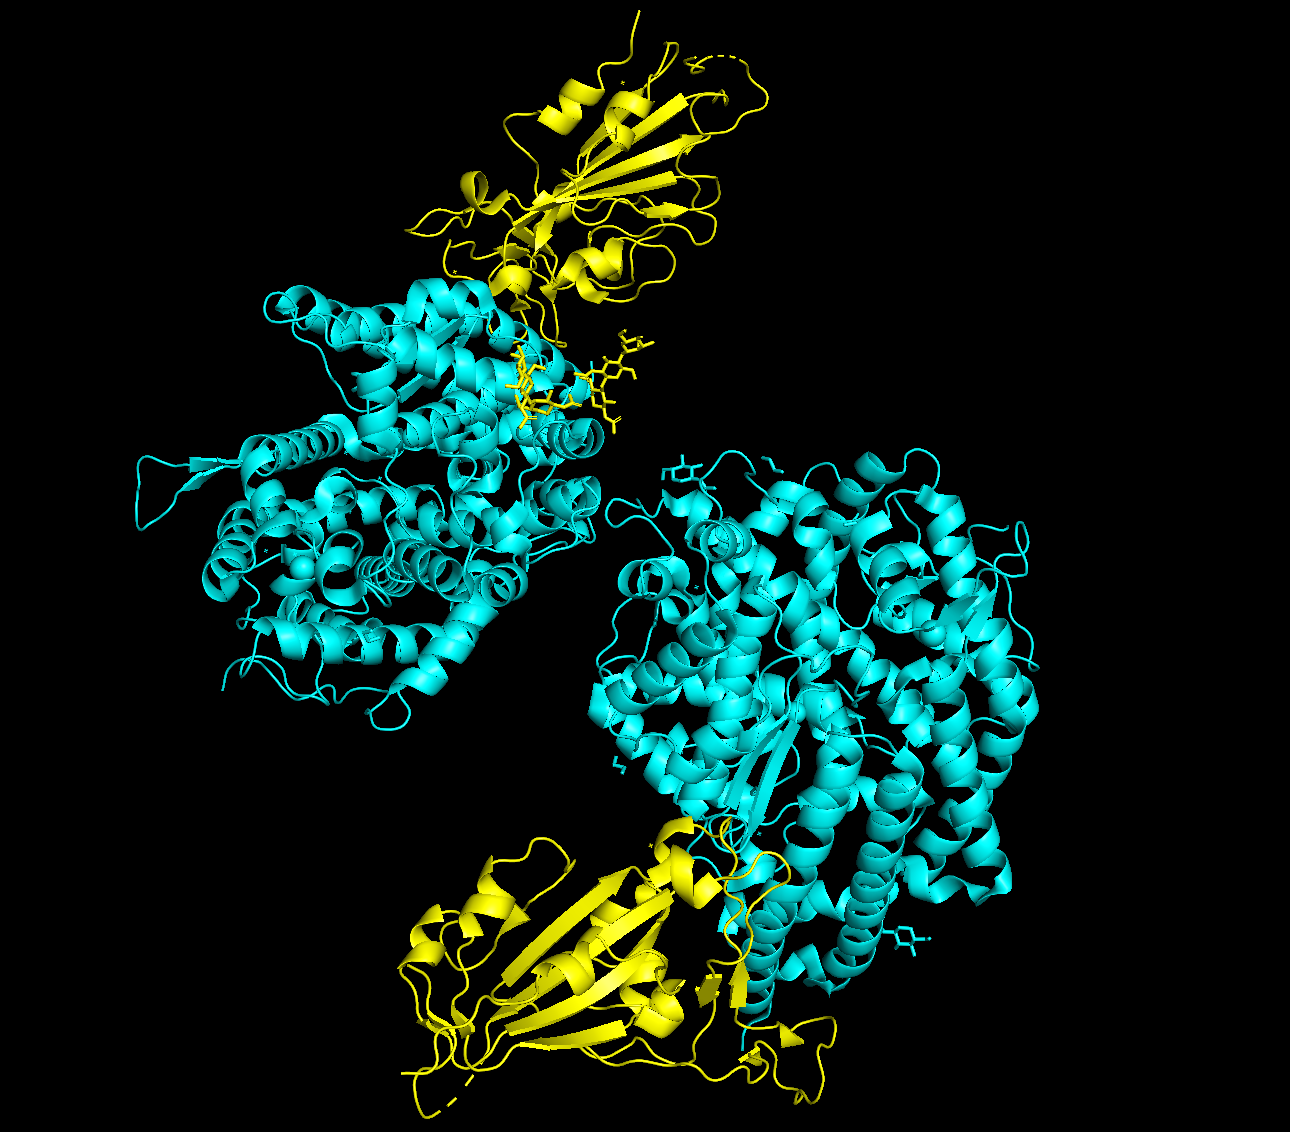
\includegraphics[width=0.8\textwidth]{figures/RBD-interaction.png}
    \figcaptionalt{Figure}{Structure of SARS-CoV-2 spike protein (yellow) complexed with its target ACE2 (cyan)}{SARS-CoV-2 spike protein complexed with its target ACE2}
\end{figure}

\subsection{Machine Learning}

Machine learning is a branch of artificial intelligence used to build models for classification or decision-making based on data, without explicit programming. Nowadays, machine learning is used across industrial fields to plan, make correct decisions, and increase the efficiency of the processes \cite{Mottaqi2021}. 

Within the field of biology, machine learning has outperformed human analysis in certain tasks. For example, in 2018, \citeauthor{Kakadiaris2018} designed a support-vector machine model for classifying risk of cardiovascular disease that produced an accuracy of over 85\% and missed fewer disease events than the US guidelines' manual risk calculator.

Despite its success, the use of machine learning within biology has been met with criticism. Models, especially black-box models (where the internal working is not revealed), have been condemned for their uninterpretable logic, and for not being paired with a biological explanation \cite{Rudin2019}. Bioinformatic problems often represent high-stakes decisions (e.g. diagnoses), so it is imperative that models used to address the problems can be trusted from a biological standpoint.

\subsection{Sequence Classification}

Proteins are biomolecules that comprise chains of organic compound units known as amino acids. There are twenty amino acids, each of which can be represented using a letter character. By defining a protein as a sequence of characters corresponding to the amino acid chain, the sequence can be used as a feature vector for classification. Take the human ACE2 sequence, built of a chain of 805 acid residues:

\[ MSSSSW...DVQTSF \]

\noindent where each letter corresponds to a distinct acid (methionine as $M$, serine as $S$, etc.). The sequence can be converted into a feature vector:

\[ x = (M,S,S,S,W,...,D,V,Q,T,S,F) \]

\noindent which can be used for classification. The features are categorical (limited to a fixed set of values) and nonordinal (there is no logical sorting order). 

The basis of this study is using the amino acid feature vectors of a protein to classify sequences as susceptible or immune to SARS-CoV-2.

\subsection{Objective and Contribution}

This study is an investigation into the validity of machine learning for classifying sequence susceptibility to SARS-CoV-2, to gain insight into the validity of machine learning as a bioinformatic tool at a higher level.

Three classification models are designed:
\begin{itemize}
    \setlength\itemsep{0em}
    \item a \textbf{baseline} machine learning model;
    \item an \textbf{eliminative} machine learning model; and
    \item a \textbf{structural} model that incorporates the findings of a protein structure analysis
\end{itemize}

The models are tested against a set of host protein sequences to evaluate their performances. It is hypothesized that the structural model will outperform its machine learning counterparts as the more accurate classifier.

\subsection{Related Work}

Machine learning has been growing in popularity for sequence classification \cite{Iqbal2014}, but an ongoing barrier is the magnitude of the feature vectors: proteins can be built of hundreds or thousands of amino acids, so reducing the problem to a manageable number of features can be challenging \cite{Saidi2010}. Bioinformaticians including \textcite{Iqbal2014} and \textcite{Saidi2010} have developed methods for feature selection specifically designed for reducing size of the feature vector of protein sequences, each leading to models that outperform standard machine learning tools.   

\textcite{Patel2016} reported linear discriminant analysis was a more accurate method than support vector machines, naive Bayes, and logistic regression when classifying amino acid sequences as secretory or not. Discriminant analysis involves applying statistical methods to find a set of features that best separates the classes \cite{Abdi2007}. The principals of discriminant analysis were implemented in the machine learning models of this study: training sequences were analyzed to identify which acids were most influential to susceptibility, and those acids were used as indicators for susceptibility in the models. 

Many studies have included structural investigations into how changes in the ACE2 sequence affects binding with the SARS-CoV-2 spike protein:
\begin{itemize}
    \setlength\itemsep{0em}
    \item In an overview of ACE2 and its function, \textcite{Li2021} reported major interaction sites including positions 24-42, 79-83, and 353-357, emphasizing positions 38, 41, 42, 82, 83, 353, and 355.
    \item \textcite{Zhao2020} investigated the effect of mutations in 23 critical sites, highlighting the effects of positions 24, 27, 30, 31, 34, 41, 79, 82, 83, 325, 329, and 353.
    \item \textcite{Luan2020} consolidated the results of existing structural analyses and used their findings to predict the host range of the virus (the set of species the virus is capable of infecting), focusing on the acids in positions 31, 35, 38, 82, and 353.
\end{itemize}
